\epigraph{\textit{It doesn't matter how beautiful your theory is, it doesn't matter how smart you are. If it doesn't agree with experiment, it's wrong.}}{-- \textup{Richard P. Feynman }}

In the following chapter, a description of the theoretical concepts needed for a proper understanding of this document is done. Ranging from \textit{knowledge graphs} to \textit{data-flow algorithms}, we are providing a firm foundation for the experiment to be conducted.

\section{Knowledge graphs}

A knowledge graph uses a graph-structured data model to represent knowledge of some real-world domain. Where each node represents an entity -- a \textit{thing} from the actual world -- and the edges are the relationships between them. This type of graph is often assembled from a wide variety of sources, and as a result, can be highly diverse in terms of structure and granularity~\cite{DBLP:journals/corr/abs-2003-02320}. To address this issue, representations of \textit{schema}, \textit{identity} and \textit{context} are needed. While the former defines the high-level structure of the graph, \textit{identity} relates nodes that conform the same real-world entity; finally, \textit{context} provides the environment for a specific knowledge to be understood. These graphs can be modelled using different technologies; however, we will focus on the most representative example of attributed ones: \textit{Wikibase graphs}.

\subsection{Wikibase graphs}

Wikidata started back in 2012 as a support to Wikipedia. Rapidly becoming one of the biggest human knowledge bases, with remarkable organizations donating their data to it; as an example, Google migrated \textit{Freebase} -- its previous knowledge graph -- to Wikidata in 2017~\cite{10.1145/2872427.2874809}. As of October 9, 2022, Wikidata currently contains roughly 100 million items\footnote{\url{https://www.wikidata.org/wiki/Wikidata:Statistics}}. Internally, Wikidata's content is stored in a SQL database (MariaDB); however, this system is not ideal for querying or data analysis. With that in mind, and pursuing the integration of Wikibase within the semantic web ecosystem, the Wikimedia Foundation adopted BlazeGraph: an open-source triple store and graph database\footnote{\url{https://en.wikipedia.org/wiki/Blazegraph}}. This way, two data models coexist in Wikibase: a document-centric model based on MediaWiki, and an RDF-based one, that can be used to perform SPARQL queries through the Query Service~\cite{https://doi.org/10.48550/arxiv.2110.11709}.

\begin{figure}[ht]
    \centering
    \includestandalone{figures/fig_02_architectureWikibase}
    \caption[Simplified architecture of Wikibase]{Simplified architecture of Wikibase~\cite{https://doi.org/10.48550/arxiv.2110.11709}}
    \label{fig:architecture:wikibase}
\end{figure}

Informally speaking, the Wikibase data model is composed by \textit{entities} and \textit{statements} (about those entities). This way, an entity can be either an \textit{item} or a \textit{property}. Items are used to represent all the \textit{things} from the human knowledge. Usually denoted by a \texttt{Q} followed by a sequence of digits; as an example, \href{https://www.wikidata.org/wiki/Q7251}{Q7251} represents Alan Turing in Wikidata. On the other hand, properties model a relationship between an item and a value, and are represented by a \texttt{P} followed by a sequence of numbers; as an example, \href{https://www.wikidata.org/wiki/Property:P31}{P31} is the property \textit{instance of} in Wikidata.

For values to be associated to properties, they must belong to some specific data type\footnote{\url{https://www.wikidata.org/wiki/Help:Data_type}}. Supported data types include: URLs, time, quantities, mathematical expressions; to name a few. Notice how more complex data types are also supported; those include \textit{properties} and \textit{items}, this way, relationships among entities are allowed.

Lastly, a statement is a piece of data about an item, and is recorded in the page of the item itself. Putting it all together, the way Wikibase manages information is as follows: through a statement, we add information to a certain item using some property and its value.

\begin{example}[Adding information to an entity in Wikidata\footnote{\url{https://www.wikidata.org/wiki/Help:Statements}}]
    In order to include information about the genre of \textit{The Hunger Games} in Wikidata, we would need to add a statement to the item itself: \href{https://www.wikidata.org/wiki/Q11679}{The Hunger Games (Q11679)}, using the property \href{https://www.wikidata.org/wiki/Property:P136}{genre (P136)}, we can then add the value \href{https://www.wikidata.org/wiki/Q15062348}{dystopian fiction (Q15062348)}. Notice how we are linking two entities (\textit{items}) of the Wikidata.
\end{example}

\begin{table}[ht]
    \centering
    \documentclass{standalone}
\usepackage[table,xcdraw]{xcolor}
\usepackage{varioref,multicol}
\usepackage{hyperref}  
\begin{document}
\begin{tabular}{|c|l|l|l|}
    \hline
    \rowcolor[HTML]{EFEFEF}
    \textbf{Language}     & \multicolumn{1}{c|}{\cellcolor[HTML]{EFEFEF}\textbf{Item}}                              & \multicolumn{1}{c|}{\cellcolor[HTML]{EFEFEF}\textbf{Property}}                            & \multicolumn{1}{c|}{\cellcolor[HTML]{EFEFEF}\textbf{Value}}                             \\ \hline
    \textit{English}      & \multicolumn{1}{l|}{\href{https://www.wikidata.org/wiki/Q11678}{The Hunger Games}}      & \multicolumn{1}{l|}{\href{https://www.wikidata.org/wiki/Property:P136}{genre}}            & \multicolumn{1}{l|}{\href{https://www.wikidata.org/wiki/Q15062348}{dystopian fiction}}  \\ \hline
    \textit{Spanish}      & \multicolumn{1}{l|}{\href{https://www.wikidata.org/wiki/Q11678}{Los juegos del hambre}} & \multicolumn{1}{l|}{\href{https://www.wikidata.org/wiki/Property:P136}{género}}           & \multicolumn{1}{l|}{\href{https://www.wikidata.org/wiki/Q15062348}{ficción distópica}}  \\ \hline
    \textit{French}       & \multicolumn{1}{l|}{ \href{https://www.wikidata.org/wiki/Q11678}{Hunger Games}}         & \multicolumn{1}{l|}{\href{https://www.wikidata.org/wiki/Property:P136}{genre artistique}} & \multicolumn{1}{l|}{\href{https://www.wikidata.org/wiki/Q15062348}{fiction dystopique}} \\ \hline
    \multicolumn{1}{l|}{} & \multicolumn{1}{c|}{\href{https://www.wikidata.org/wiki/Q11678}{Q11678}}                & \multicolumn{1}{c|}{\href{https://www.wikidata.org/wiki/Property:P136}{P136}}             & \multicolumn{1}{c|}{\href{https://www.wikidata.org/wiki/Q15062348}{Q15062348} }         \\ \cline{2-4}
\end{tabular}
\end{document}
    \caption[Including information about the genre of \textit{The Hunger Games}]{Including information about the genre of \textit{The Hunger Games}\footnotemark}
    \label{tab:language}
\end{table}
\footnotetext{\url{https://www.wikidata.org/wiki/Q11678}}

\begin{figure}[ht]
    \centering
    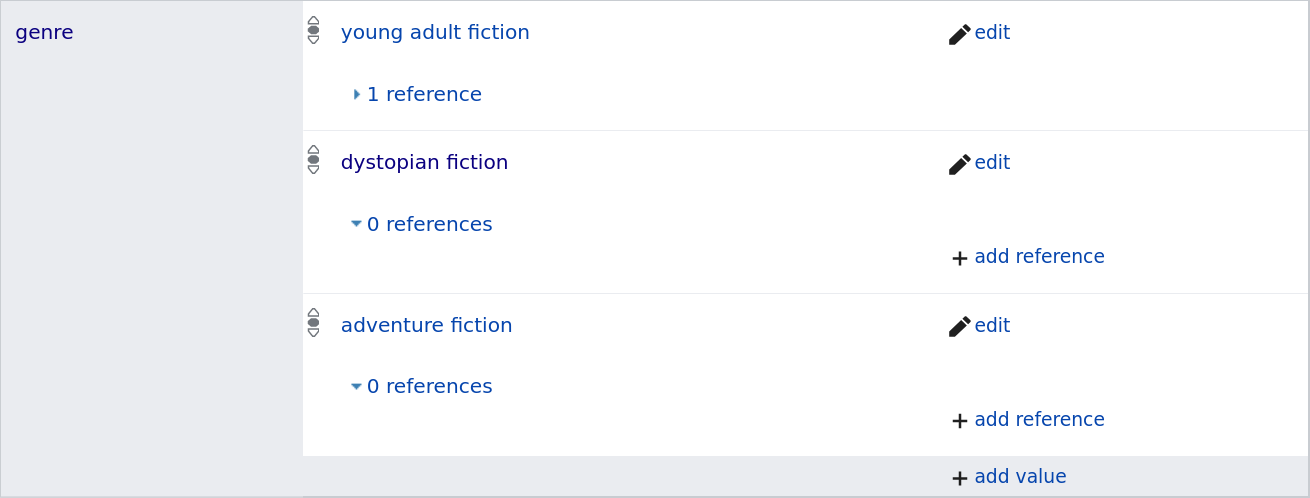
\includegraphics[width=\textwidth]{../img/wikidata_statement.png}
    \caption[Example of a simple statement annotating the genre of \textit{The Hunger Games}]{Example of a simple statement annotating the genre of \textit{The Hunger Games}\footnote{\url{https://www.wikidata.org/wiki/Q11678}}}
    \vspace{-3mm}
\end{figure}

\subsubsection{Opaque URIs}

As noted above, the main purpose of Wikidata is to store data about things that are described by pages in Wikipedia (in any language)\footnote{\url{https://www.mediawiki.org/wiki/Wikibase/DataModel}}. This means, \textit{things} should be represented in such a way that they don't depend on the natural language used; that is, language independence is required. In Wikidata, this is achieved through a linked data pattern called \textit{opaque URIs}. In general, a URI is defined as a unique sequence of characters that identifies the resources of the system\footnote{\url{https://en.wikipedia.org/wiki/Uniform_Resource_Identifier}}. Designing good URIs is the first step in a linked data development.

The characters that appear in a URI tend to be related to the concept they represent, improving human-readability. As an example, \texttt{https://example.com/España} could -- potentially -- be an identifier for the Spanish country. However, for those non-Spanish speakers, that identifier is meaningless. What's more, the use of non-ASCII characters may lead to problems in an internationalized system. Opposed to \textit{descriptive URIs}, \textit{opaque} ones are not intended to represent terms in a natural language~\cite{LabraGayo2015MultilingualLD}. An example to that is: \url{https://www.wikidata.org/wiki/Q11679}, where item \texttt{Q11679} represents \textit{The Hunger Games} in Wikidata. However -- under some situations -- it is handful for users to interact with human-readable names. In Wikidata, this is solved through \textit{labels}, which are language-dependent. Following the previous example, the label tagged to the entity \texttt{Q11679} is the actual title of the book: \textit{The Hunger Games}. Translations for several languages can also be provided. Notice Table~\ref{tab:language} for an example of possible \textit{labels} for some \textit{opaque URIs}.

What we have seen so far is an overview of the Wikibase \textit{data model}; including: \textit{statements}, \textit{properties}, \textit{values} and the appropriate mechanism for identifying them (in a multilingual approach). Putting it all together, the next step is to formally define a Wikibase graph.

\begin{definition}[Wikibase graph~\cite{https://doi.org/10.48550/arxiv.2110.11709}]
    Given a mutually disjoint set of items \ItemSet{}, a set of properties \PropSet{} and a set of data values \DataValueSet{}, a \emph{Wikibase graph} is a tuple $\langle\ItemSet,\PropSet,\DataValueSet,\StmtSet\rangle$ such that $\StmtSet\subseteq\EntitySet\times\PropSet\times\ValueSet\times\FinSet{\PropSet\times\ValueSet}$ where $\EntitySet=\ItemSet\cup\PropSet$ is the set of entities which can be subjects of a statement and $\ValueSet=\EntitySet\cup\DataValueSet$ is the set of possible values of a property.
\end{definition}

For a better understanding  of this formal definition, let me explain it step-by-step. First, let us clarify what the described symbols are: $\mathcal{Q}$ is the set containing the different entities (\textit{things}), $\mathcal{P}$ is the set with the different possible relationships in the graph, $\mathcal{D}$ is the set containing data values and $\rho$ is the set where relationships among the previous elements are annotated. This way, through the relationships in $\mathcal{P}$, we can add information ($\mathcal{Q}$, $\mathcal{P}$ or $\mathcal{D}$) to any item in $\mathcal{Q}$. Lastly, $\mathcal{V}$ provides extra information to a certain relationship. This is useful when you want to include more data to a particular statement; as an example, in order to establish the \href{https://www.wikidata.org/wiki/Property:P585}{point in time} at which \href{https://www.wikidata.org/wiki/Q937}{Albert Einstein} received the \href{https://www.wikidata.org/wiki/Q38104}{Nobel Prize in Physics}, we may annotate the \href{https://www.wikidata.org/wiki/Property:P166}{award received} property with the value 1921\footnote{\url{https://www.nobelprize.org/prizes/physics/1921/summary/}}. Those are called \textit{qualifiers}. For further clarifications, let us model the Wikibase graph of a certain scenario.

\begin{example}
    We are willing to qualify that Alan Turing (23 June 1912 -- 7 June 1954) was employed by the government of the United Kingdom in the course of the WWII. During that time he invented a computer for deciphering Enigma-machine-encrypted secret messages\footnote{\url{https://en.wikipedia.org/wiki/Bombe}}. Additional information about relevant places where he lived is also annotated.
\end{example}

\begin{table}[h]
    \vspace{-2mm}
    \centering
    % Longatable File '01_tab_wikibaseGraph.tex'
\documentclass{standalone}
\usepackage{longtable}
\newcommand{\myfont}[1]{\ensuremath{\mathcal{#1}}}

\newcommand{\triple}[3]{\ensuremath{\langle #1,#2,#3 \rangle}}
\newcommand{\quadruple}[4]{\ensuremath{\langle #1,#2,#3,#4\rangle}}

\newcommand{\ItemSet}{\myfont{Q}}
\newcommand{\PropSet}{\myfont{P}}
\newcommand{\EntitySet}{\myfont{E}}
\newcommand{\ValueSet}{\myfont{V}}
\newcommand{\DataValueSet}{\myfont{D}}
\newcommand{\StmtSet}{\rho}
\newcommand{\FinSet}[1]{\ensuremath{FinSet(#1)}}

\newcommand{\hrefc}[3][blue]{\href{#2}{\color{#1}{#3}}}%

\newcommand{\elemento}[2]{\ensuremath{\hrefc[violet]{http://www.wikidata.org/entity/#2}{#1}}}
\newcommand{\propiedad}[2]{\ensuremath{\hrefc[blue]{http://www.wikidata.org/entity/#2}{#1}}}
\newcommand{\alanTuring}{\elemento{alanTuring}{Q7251}}
\newcommand{\wilmslow}{\elemento{wilmslow}{Q2011497}}
\newcommand{\town}{\elemento{town}{Q3957}}
\newcommand{\government}{\elemento{government}{Q220798}}
\newcommand{\warringtonLodge}{\elemento{warringtonLodge}{Q20895942}}
\newcommand{\bombe}{\elemento{bombe}{Q480476}}
\newcommand{\unitedKingdom}{\elemento{unitedKingdom}{Q145}}
\newcommand{\computer}{\elemento{computer}{Q11742076}}
\newcommand{\dateOfBirth}{\propiedad{dateOfBirth}{P569}}
\newcommand{\placeOfBirth}{\propiedad{placeOfBirth}{P19}}
\newcommand{\country}{\propiedad{country}{P27}}
\newcommand{\employer}{\propiedad{employer}{P108}}
\newcommand{\discoverer}{\propiedad{discoverer}{P61}}
\newcommand{\dateOfDeath}{\propiedad{dateOfDeath}{P570}}
\newcommand{\placeOfDeath}{\propiedad{placeOfDeath}{P20}}
\newcommand{\timeStart}{\propiedad{timeStart}{P580}}
\newcommand{\timeEnd}{\propiedad{timeEnd}{P582}}
\newcommand{\manufacturer}{\propiedad{manufacturer}{P176}}
\newcommand{\Human}{\elemento{Human}{Q5}}
\newcommand{\instanceOf}{\propiedad{instanceOf}{P31}}

\setlength{\tabcolsep}{1mm}
\renewcommand{\arraystretch}{1.5}
\begin{document}
\begin{longtable}{ccl}
    \caption{Example of a Wikibase graph according to its definition}
    \label{tab:wikibase:graph}
    \endlastfoot
    \ItemSet      & = \{ & \alanTuring, \wilmslow, \government, \unitedKingdom, \warringtonLodge,                           \\
                  &      & \bombe, \town, \computer \hspace{1mm} \}                                                         \\
    \PropSet      & = \{ & \dateOfBirth, \placeOfBirth, \employer, \dateOfDeath, \placeOfDeath,                             \\
                  &      & \timeStart, \country, \timeEnd, \manufacturer, \instanceOf \hspace{1mm} \}                       \\
    \DataValueSet & = \{ & {\small 23 June 1912}, {\small 7 June 1954}, {\small 1938}, {\small 1945}\hspace{1mm} \}         \\
    $\StmtSet$    & = \{ & (\alanTuring, \instanceOf, \Human, \{\}),                                                        \\
                  &      & (\alanTuring, \dateOfBirth, {\small 23 June 1912}, \{\}),                                        \\
                  &      & (\alanTuring, \placeOfBirth, \warringtonLodge, \{\}),                                            \\
                  &      & (\alanTuring, \dateOfDeath, {\small 7 June 1954}, \{\}),                                         \\
                  &      & (\alanTuring, \placeOfDeath, \wilmslow, \{\}),                                                   \\
                  &      & (\alanTuring, \employer, \government, \{ \timeStart: {\small 1938}, \timeEnd: {\small 1945} \}), \\
                  &      & (\bombe, \discoverer, \alanTuring, \{\}),                                                        \\
                  &      & (\bombe, \manufacturer, \government, \{\}),                                                      \\
                  &      & (\bombe, \instanceOf, \computer, \{\}),                                                          \\
                  &      & (\bombe, \country, \unitedKingdom, \{\})                                                         \\
                  &      & (\wilmslow, \country, \unitedKingdom, \{\})                                                      \\
                  &      & (\wilmslow, \instanceOf, \town, \{\})                                                            \\
                  &      & (\warringtonLodge, \country, \unitedKingdom, \{\})\hspace{1mm} \}                                \\
\end{longtable}
\end{document}
\end{table}

\begin{figure}[H]
    \centering
    \includestandalone[width=0.9\textwidth]{figures/fig_03_wikibaseGraph}
    \caption[Formal description and visualization of Turing's Wikibase graph]{Formal description and visualization of Turing's Wikibase graph}
\end{figure}

\subsubsection{Wikibase data serialization}

The Wikibase data model supports two export formats: JSON and RDF. Being the former the one employed by the JSON dumps and the latter follows semantic web and linked data principles. A fragment of both formats is shown below.

\begin{example}[Seralization of a node using JSON and RDF]
    \href{https://www.wikidata.org/wiki/Q7251}{Alan Turing (Q7251)} was \href{https://www.wikidata.org/wiki/Property:P108}{employed (P108)} by the \href{https://www.wikidata.org/wiki/Q220798}{Government Communications Headquarters (Q220798)} of the United Kingdom, during the World War II (1938-1945).
\end{example}

\paragraph{Wikibase JSON serialization}

The JSON serialization follows the Wikibase data model~\cite{https://doi.org/10.48550/arxiv.2110.11709}. Consisting of a sequence of items where each element is a JSON object capturing all the information about the item itself, represented in a single line. What's remarkable of this mechanism is that it records all the neighboring entities of every single node, making the algorithms validating whole graphs able to process them in a single pass. More on this will be discussed in paragraph \ref{section:pregel}.

\begin{lstlisting}[style=JSON]
[
    { "type": "item", "id": "Q42", "claims": { "P31": [...
    { "type": "item", "id": "Q80", "claims": { "P108": [...
    { "type": "property", "id": "P108", "claims": { ... 
    ... 
]
\end{lstlisting}

\paragraph[Wikibase RDF serialization]{Wikibase RDF serialization\footnotemark}
\footnotetext{\url{https://www.wikidata.org/wiki/Special:EntityData/Q7251.ttl}}

The RDF serialization of Wikidata\footnote{\url{https://www.mediawiki.org/wiki/Wikibase/Indexing/RDF_Dump_Format}} is mainly used by the Wikidata's Query Service described above (see figure \ref{fig:architecture:wikibase}). The main goal of this formatting is providing support to semantic web technologies.

\begin{lstlisting}[style=Turtle]
wd:Q7251 p:P108 s:Q7251-5c5c1b1c-40a4-b9c0-40a6-dfaccd56f273 .

s:Q7251-5c5c1b1c-40a4-b9c0-40a6-dfaccd56f273 a wikibase:Statement,
wikibase:BestRank ;
wikibase:rank wikibase:NormalRank ;
ps:P108 wd:Q220798 ;
pq:P580 "1938-01-01T00:00:00Z"^^xsd:dateTime ;
pqv:P580 v:560845b053d80d9ba30cc757808172fd ;
pq:P582 "1945-01-01T00:00:00Z"^^xsd:dateTime ;
pqv:P582 v:db243e11a2e2c6bb034f59e082f66d29 ;
prov:wasDerivedFrom ref:7d58b689209415697990098179e8ace8b04630a1 .
\end{lstlisting}

\section{Data-flow algorithms}

The main focus of this document is implementing a Big data solution using the Pregel algorithm. However, for better understanding it, introducing the MapReduce model will be handful. Notice that both are meant to be executed in parallel in a distributed system.

\subsection{MapReduce}

Inspired by the map and reduce functions, a MapReduce~\cite{wiki:MapReduce} program is composed of a \textit{map procedure}, where we apply a simple operation to all the elements of a sequence, followed by a \textit{reduce} method, which transforms those elements into a single result. For us to process a graph, we would need to chain MapReduce invocations. Where, for each iteration, map and reduce functions are applied. The main drawback of this approach, is the functional nature of the MapReduce model. This means, expressing a graph algorithm as a chained MapReduce results in having to pass the entire state of the graph from one stage to another~\cite{10.1145/1807167.1807184} .

\subsection{Pregel model}
\label{section:pregel}

Pregel (\textit{Parallel, Graph and Google}) is a data flow paradigm and system created by Google to handle large-scale graphs. Even though the original system remains proprietary at Google, the computational model was adopted by many graph-processing systems: including Apache Spark. For better understanding Pregel, the idea is to \textit{think like a vertex}; this way, for computing the state of a given node, we only depend on the states of its neighboring ones. We will call neighboring vertices of a certain one to those nodes connected to it by an outgoing edge. This has a relevance for better understanding the architecture of this system depicted in Figure \ref{fig:architecture:pregel}. \textit{Thinking like a vertex} could be understood as the \textit{leitmotif} for dividing the problem into several sub-problems: instead of dealing with a huge graph, we just have to solve the problem for smaller graphs: a vertex and its neighboring ones. Notice how a graph to be processed with Pregel may potentially have millions of vertices with billions of edges. More on the size of the Wikibase graphs will be discussed later on.

In comparison to the MapReduce framework, where for each iteration the state of the whole graph must be passed, at each \textit{superstep} -- the way we refer to iterations in Pregel -- each vertex can: send a message to its neighbors, process the received messages (from the previous superstep), and update its state. Summing up, instead of sending the whole state of the graph, we just send messages back and forth. The best way for understanding this is through an example. Let me show you the resulting trace after applying Pregel for computing the maximum value in a graph (see figure \ref{fig:pregel}).

\begin{figure}[ht]
    \centering
    \includestandalone{figures/fig_04_pregelTrace}
    \caption[Trace of the execution of Pregel for computing the maximum value]{Trace of the execution of Pregel for computing the maximum value~\cite{10.1145/1807167.1807184}}
    \label{fig:pregel}
\end{figure}

Notice that at the beginning of the execution, the state of all the nodes will be set to active. This initial stage is called \textit{superstep 0}. When a vertex is active, it sends a message to its neighbors, that will receive it in the next \textit{superstep}. In this case, the message we are propagating is the largest value that we have learned so far. As an example to that, the second to the left node starts with a value of 6 -- which is the maximum value of the graph -- and sends that number to its neighbors: 3 and 1. In the next \textit{superstep}, the vertices that have received a message have to compare both: the value they store and the received one. This comparison is what it's called the \textit{vprog} function, which will vary from one problem to another. Then, both nodes will update its state to 6. As they have updated their state, they will have to send the new value to its neighbors: beginning another iteration (\textit{superstep}). Notice that at the \textit{superstep 1}, the second to the left node is halted as it doesn't send any other message to its neighbors as it's value has not changed. When every node is halted -- inactive -- the execution of the algorithm finishes. In the figure \ref{fig:state} a simplified state machine is shown.

\begin{figure}[ht]
    \centering
    \includestandalone{figures/fig_05_stateDiagram}
    \caption[Simplified state diagram of a vertex]{Simplified state diagram of a vertex~\cite{10.1145/1807167.1807184}}
    \label{fig:state}
\end{figure}

\subsubsection{Architecture of a Pregel system}

It's quite simple to describe the architecture of a Pregel system. As we have seen, one of the main goals of this algorithm is achieving a parallel execution. This way, a \textit{master} node will divide the graph into several partitions and assign one (or more) of them to each \textit{worker} node. For the \textit{master} to create the partitions it selects a bunch of vertices and all those vertices' outgoing edges; remember: \textit{think like a vertex}.

\begin{figure}[ht]
    \centering
    \includestandalone{figures/fig_06_pregelArchitecture}
    \caption[Architecture of a Pregel system]{Architecture of a Pregel system~\cite{10.1145/3349265}}
    \label{fig:architecture:pregel}
\end{figure}

\section{Knowledge graph validation}